\documentclass[a4paper, 12pt]{article}

\usepackage{wrapfig}
\usepackage{graphicx}
\usepackage{mathtext}
\usepackage{amsmath}
\usepackage{siunitx}
\usepackage{multirow}
\usepackage{rotating}

\usepackage[T1,T2A]{fontenc}

\usepackage[russian]{babel}

\graphicspath{{pictures/}}


\title{\begin{center}Лабораторная работа №2.1.3\end{center}
Определение $C_p/C_v$ по скорости звука в газе}
\author{Гёлецян А.Г.}
\date{\today}

\begin{document}
    \pagenumbering{gobble}
    \maketitle
    \newpage
    \pagenumbering{arabic}

    \section{Цель работы}
    Определение показателя адиабаты с помощью уравнения состояния идеального газа.

    \section{Теория}
    \paragraph{}
    Скорость распостранения звука в идеальных газах определяется формулой
    \[c=\sqrt{\gamma\frac{RT}{\mu}}\]
    где $R$ - газовая постоянная, $T$ - температура газа, $\mu$ - его молярная масса.
    \paragraph{}
    Преобразуя формулу найдем

    \begin{equation}
        \gamma=\frac{\mu}{RT}c^2
    \end{equation}

    \paragraph{}
    Как видим, чтобы найти показатель адиабаты надо измерить скорость звука в идеальном при разных температурах. Для измерения скорости звука воспользуемся установкой, изображенной на рис. 1
    \begin{figure}[h]
        \begin{center}
            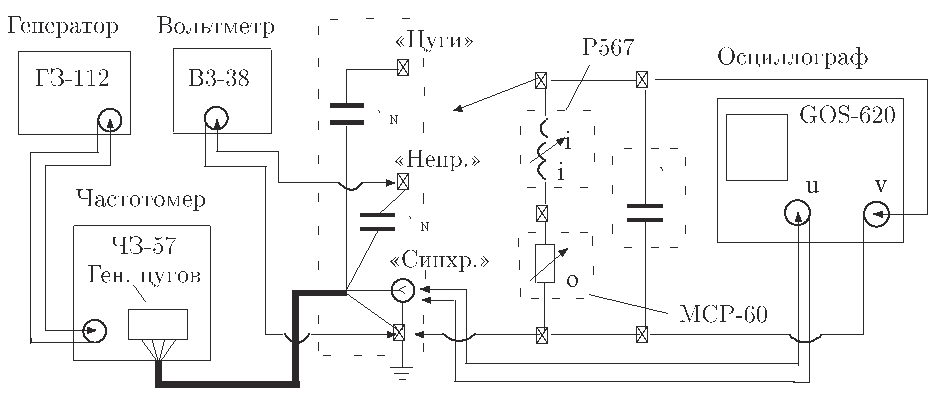
\includegraphics[width=0.8\linewidth]{ustanovka}
            \caption{Схема установки}
        \end{center}
    \end{figure}

    Термостат обеспечивает постоянную температуру газа внутри трубы во время опыта.
    Подстраивая частоту генератора звука добьемся максимума амплитуды сигнала на
    осциллографе. Эти максимумы соответствуют гармоникам трубы, т.е. тем ситуациям,
    когда на длину трубы приходиться целое число полуволн звука. Если обозначить длины
    трубы и волны $L$ и $\lambda$ соответственно, то гармоникам соответсуют длины волны
    \[\lambda_n=\frac{2L}{n}\]
    Использовав соотношение $c=\lambda\nu$
    \begin{equation}
        c=2L\frac{\nu_n}{n}
    \end{equation}

    \section{Ход работы}
    Согласно теории проведем измерения частот первых пяти гармоник в прямом и обатном
    направлениях. Устонавливаем на термостате нужную температуру (в измерениях при
    комнатной температуре термостат был выключен) и ждем несколько минут чтобы
    минимизмровать различие между температурами газа в трубе и воды в термостате.
    Результаты измерении приведены в таблице ниже.

    \begin{table}[h]
        \begin{center}
            \begin{tabular}{|c|r|r|r|r|}
                \hline
                {$T, К$} &   296К &  303.3К &  313.2К &  323.2К \\
                \hline
                $\nu_1, Гц$ &   256 &    272 &    275 &    264 \\\hline
                $\nu_2, Гц$ &   497 &    503 &    510 &    517 \\\hline
                $\nu_3, Гц$ &   742 &    751 &    765 &    771 \\\hline
                $\nu_4, Гц$ &   986 &   1000 &   1016 &   1030 \\\hline
                $\nu_5, Гц$ &  1231 &   1254 &   1266 &   1291 \\\hline
                $\nu_4, Гц$ &   993 &   1000 &   1013 &   1029 \\\hline
                $\nu_3, Гц$ &   746 &    746 &    760 &    772 \\\hline
                $\nu_2, Гц$ &   495 &    502 &    510 &    519 \\\hline
                $\nu_1, Гц$ &   263 &    276 &    273 &    264 \\\hline
            \end{tabular}
        \end{center}
        \caption{Данные измерений}
    \end{table}

    Для нашей установки $L = (700 \pm 1)мм$. Погрешность округления частот равна $\Delta\nu_{ок}=1Гц$. Точность нахождения пика резонанса зависит не только от точности измерения самой частоты, а так же от самой ширины пика. При маленькой добротности пик резонансной кривой широкий, и найти точно середину бывает сложно. При слишком больших добротностях пик слишком узкий, и поймать еге с помощью грубой настройки частоты не получается. Собственно поэтому и измерения заканчиваются на пятой гармонике. Исследуя ширины разных пиков можно оценить случайные ошибки резонансных частот для разных гармоник (см. таблицу ниже).

    \begin{table}[h]
        \begin{center}
            \begin{tabular}{|c|r|r|r|r|r|}
                \hline
                {№ гармоники} &            1 &  2 &  3 &  4 & 5 \\
                \hline
                $\Delta\nu_{случ}, Гц$ &   5 &  3 &  3 &  3 & 3 \\\hline
            \end{tabular}
        \end{center}
        \caption{Случайные ошибки резонансных частот разных гармоник}
    \end{table}

    \paragraph{}
    Чтобы найти скорость звука при данной температуре построим график зависимости $2L\nu_n(n)$. Тогда, если аппроксимировать наши данные линией, то угловой коэффицент будет скорости звука. Для каждой температуры построим соответствующий график и сделаем аппроксимацию. Метрикой для минимизации был выбран $\chi^2$, которая для точек с координатами $(x_i, y_i)$ и ошибакми $\Delta x_i\approx 0, \Delta y_i$ равна
    \begin{equation}
        \chi^2(\theta) = \sum_{i}^{} \left(\frac{y_i-f(x_i| \theta)}{\Delta y_i}\right)^2
    \end{equation}
    Где $f$ это функция аппроксимации зависающая от параметров $\theta$. Предпочтение было отдано данному в попытке учесть различие ошибок резонансных частот.

    \paragraph{}
    В нашем случае $x=n, y=2L\nu_n$ а ошибки $y$ вычисляются по формуле

    \begin{equation}
        \Delta y_i = y_i \sqrt{
        \left(\frac{{\Delta\nu_{случ}}^2 + {\Delta\nu_{ок}}^2}{\nu_n^2}\right) +
        \left(\frac{\Delta L}{L}\right)^2}
    \end{equation}

    Сделав соответствующие расчеты получаем

    \begin{table}[h]
        \begin{center}
            \begin{tabular}{|c|r|r|r|r|r|}
                \hline
                {$T, К$} &   296К &  303.3К &  313.2К &  323.2К \\\hline
                {$c, мс^{-1}$} &   342.4 & 346.0 & 350.1 & 359.1 \\\hline
                {$\Delta c, мс^{-1}$} &   0.9 &  0.9 &  0.9 &  0.9 \\\hline
            \end{tabular}
        \end{center}
        \caption{Скорости звука при различных температурах}
    \end{table}

    \begin{figure}[t]
        \includegraphics[width=\textwidth]{speed_of_sound_plots}
        \caption{Графики зависимостей $2L\nu_n(n)$ при разных $T$}
    \end{figure}

    Теперь имея все эти данные посчитаем показатели адиабаты для разных температур по формуле (1), использовав значение $\mu/R=0.0034843Км^{-2}с^2$


    \begin{table}[h]
        \begin{center}
            \begin{tabular}{|c|r|r|r|r|r|}
                \hline
                {$T, К$} &   296К &  303.3К &  313.2К &  323.2К \\\hline
                {$\gamma$} &   1.38 & 1.38 & 1.36 & 1.39 \\\hline
            \end{tabular}
        \end{center}
        \caption{Показатели адиабаты при разных температурах}
    \end{table}

    Посчитав среднее и среднеквадратичное отклонение получим

    \begin{equation}
        \gamma = 1.38 \pm 0.01
    \end{equation}

    \section{Заключение}
    Полученная нами величина довольно близка к ожидаемому значению 1.4, хоть и немного заниженная.
    Различие могло возникнуть из-за наличия в воздухе одноатомных и многоатомных газов.
\end{document}


